\documentclass[12pt]{article}

\usepackage[dutch]{babel}
\usepackage{a4wide}
\usepackage{amsmath}
\usepackage{enumerate}
\usepackage{eurosym}
\usepackage{url}
\usepackage{graphicx}
\usepackage{hyperref}

\author{Jos Bonsink \& Mustafa Karaalioglu}

\begin{document}

\title{Hoe precies kan er realtime een Android-apparaat akoestisch gelokaliseerd worden?}
\maketitle

\section{Inleiding}
Aan het begin van het Net-Centric Computing project hadden enkele groepen besloten met robots te gaan werken. Hierbij was het nodig om realtime de lokale posities van de robots te kunnen bepalen. Tegenwoordig wordt positiebepaling voornamelijk gedaan met behulp van GPS. Echter, is dit niet overal beschikbaar. Tevens is GPS slechts nauwkeurig tot op enkele meters. GPS is dus niet geschikt voor positiebepaling in kleine ruimtes. Andere groepen kozen ervoor om gebruik te maken van \textit{image vision} waar de robots altijd in beeld moet zijn. Dit artikel onderzoekt de mogelijkheden om realtime \cite{stankovic1988misconceptions} posities akoestisch te bepalen.

Er is reeds onderzoek gedaan naar de applicatie van geluid om positie te bepalen. Enzo Mumolo, Massimiliano Nolich en Gianni Vercelli hadden een algoritme ontwikkeld voor realtime lokalisatie voor het gebruik van een microfoonarray in luidruchtige omstandigheden. Zij haalden een precisie van ongeveer 20 cm voor 90\% van alle gevallen in luidruchtige omstandigheden \cite{mumolo2003algorithms}. Een microfoonarray plaatsen op een robot is duur en log. Er is ook onderzoek geweest naar goedkopere oplossingen zoals een telefoon. 

Microsoft Asia had onderzoek gepleegd naar het gebruik van telefoons om afstanden te bepalen. Ze hadden een algoritme ontwikkeld dat tot een paar centimeter precies was in stille omgevingen \cite{peng2007beepbeep}. Vervolgonderzoek breidde dit uit tot volledige positiebepaling met behulp van geluid en andere sensoren zoals een gyroscoop. Zij behaalden een nauwkeurigheid van 13.9 cm voor 90\% van de gevallen \cite{qiu2011feasibility}.

Zou dit preciezer kunnen? Hoe precies kan er realtime een Android-apparaat akoestisch gelokaliseerd worden? De verwachting is dat een nauwkeurigheid van 10 cm te behalen moet zijn. Dit is gebaseerd op de volgende feiten: de samplerate van een microfoon is 44100 Hz, de geluidssnelheid is 340 meter per seconde. Het vermoeden is dat een piepgeluid binnen 25 samples herkend kan worden. Dit vertaalt zich naar een precisie van 10 cm.

Er zal een Android-applicatie worden ontwikkeld waarin realtime piepgeluiden gegenereerd en gedetecteerd kunnen worden binnen 25 samples. Het artikel is als volgt ingedeeld: paragraaf \ref{sec:materialen} beschrijft de gebruikte materialen en ontwikkelde methoden om realtime accurate akoestische lokalisatie uit te voeren, in paragraaf \ref{sec:resultaten} worden de resultaten getoond en tot slot worden in paragraaf \ref{sec:discussie} de resultaten ge\"evalueerd en enkele conclusies getrokken.

\section{Materialen en methoden}
\label{sec:materialen}
De experimenten met de Android-applicatie werden uitgevoerd op HTC Desire C telefoons met Android 4.0.2. Om positiebepaling mogelijk te maken met deze telefoons moesten er drie problemen worden opgelost: Bluetooth communicatie, audio detectie en afstandsmeting.

\subsection{Bluetooth}
Er zijn minstens drie Android-apparaten nodig om lokaal de positie van \'e\'en Android-apparaat te kunnen bepalen. De benodigde communicatie verliep via een peer-to-peer \cite{schollmeier2001definition} netwerk van Bluetooth \cite{haartsen2000bluetooth} verbindingen.

\begin{figure}[h]
\centering
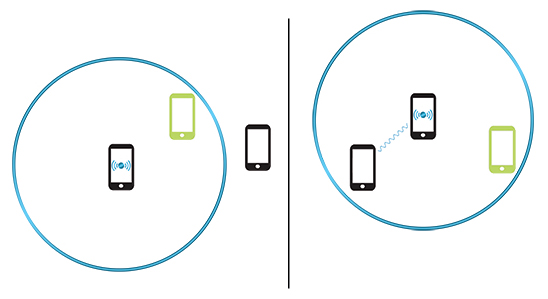
\includegraphics[scale=0.5]{bluetooth}
\caption{opzetten van peer-to-peer Bluetooth-netwerk}
\label{fig:bt}
\end{figure}

Alle deelnemende apparaten moesten op \textit{Bluetooth Discoverable} worden gezet voor een oneindige periode.
Het proces startte bij \'e\'en node die zocht naar naburige Bluetooth apparaten, ge\"illustreerd in figuur \ref{fig:bt}, met het Bluetooth Discovery proces.
Dit proces werd telkens gestopt wanneer er \'e\'en apparaat werd gevonden. Vervolgens werd er geprobeerd met dit apparaat te verbinden, in figuur \ref{fig:bt} ge\"ilustreerd als de groene telefoon. Als dit mislukte, werd Bluetooth Discovery opnieuw opgestart.

Indien het verbinden van beide apparaten was geslaagd, werd Bluetooth Discoverable uitgezet. De laatst toegevoegde node ging zoeken naar nieuwe toevoegingen voor het netwerk. Dit proces herhaalde zich totdat er na een aantal Bluetooth Discoveries geen nieuwe apparaten waren gevonden. Hierna was het dus niet meer mogelijk om het netwerk uit te breiden. Alle nodes in het netwerk waren niet meer Discoverable.

Elke nieuwe node in het netwerk ontving van zijn \textit{parent} een lijst met de reeds bekende mac-adressen. De node voegde zijn eigen mac-adres aan deze lijst toe. Vervolgens stuurde hij zijn eigen mac-adres naar zijn parent, die dit adres aan zijn eigen lijst toevoegde. Het mac-adres propageerde door het netwerk totdat het mac-adres bij de root node was terechtgekomen. Een lijst van alle mac-adressen was gelijk en beschikbaar op elk apparaat. 

\subsection{Audio detectie}
Voor het realtime detecteren van piepgeluiden moest er constant geluid opgenomen \'en geanalyseerd worden. De audiohardware bufferde continu een halve seconde aan audio. In een aparte thread werden er steeds twintig samples uit deze buffer opgehaald. Op deze samples werd een Fast Fourier Transformatie(FFT) \cite{bracewell1986fourier} toegepast. Hiermee werd het geluidssignaal als functie van tijd omgezet naar een complexe functie van amplitude en fase als functie van frequentie. 

De gegenereerde piepgeluiden bestonden uit een sinuso\"ide met een frequentie van $8820$ Hz. Na de FFT werd de lengte van het complexe getal corresponderend met de frequentie van het piepgeluid vergeleken met een drempelwaarde. Wanneer de lengte de drempelwaarde overschreed, werd het geluid herkend als een piep.

\begin{figure}[t]
\centering
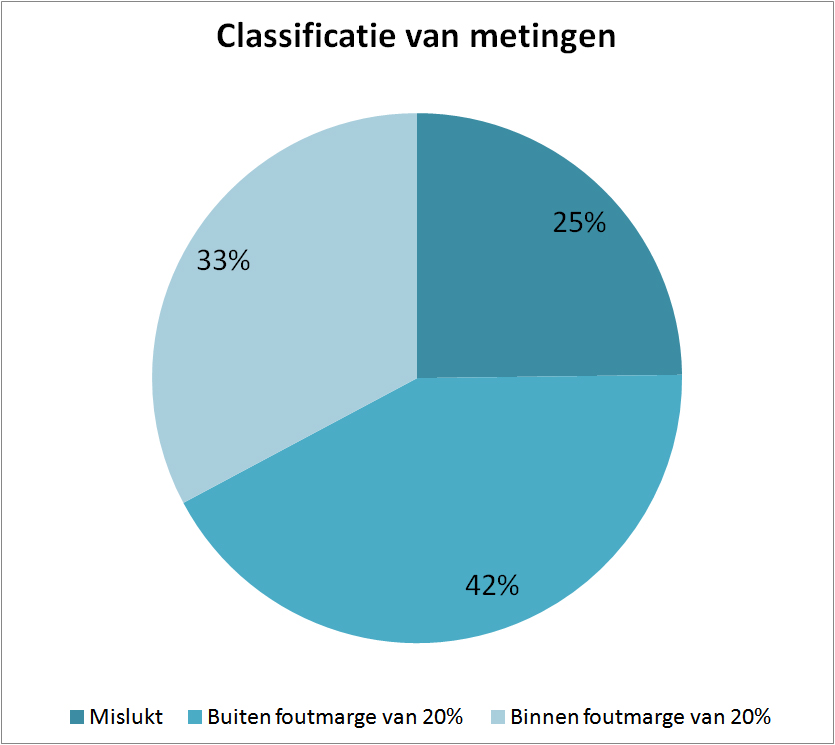
\includegraphics[scale=0.4]{classificatie}
\caption{classificatie van meetpogingen.}
\label{fig:classi}
\end{figure}


\subsection{Afstandsmeting}
De afstand tussen twee Android-apparaten werd bepaald door het tijdsverschil tussen het verzenden en ontvangen van gegenereerde piepgeluiden te meten. Uit de eerder genoemde lijst van mac-adressen in het Bluetooth-netwerk werden een \textit{master} en \textit{slave} uitgekozen aan de hand van de volgorde van de lijst. De master verzocht via Bluetooth de slave te antwoorden op zijn piepgeluid. Na bevestiging van de slave, speelde de master een piepgeluid af.

Het tijdsverschil tussen het versturen en ontvangen van piepgeluiden kon worden gemeten door het aantal samples tussen twee piepgeluiden te gebruiken. Het twee keer achterelkaar detecteren van hetzelfde piepgeluid, werd voorkomen door een korte periode na een detectie niks te detecteren. De looptijd kon exact worden verkregen door te corrigeren voor de verwerkingstijd die nodig is bij het afspelen van geluid. Voor de master werd het aantal samples tussen de detectie van zijn eigen piep en dat van de respons gemeten. Bij de slave werd het verschil gemeten tussen de detectie van het eerste piepgeluid en dat van zichzelf. Dit verschil werd via Bluetooth naar de master verstuurd. De master trok deze waarde af van de gemeten totaal aantal samples tussen de twee piepgeluiden. Aan de hand van de samplerate (44100Hz) kon de tijdsduur worden bepaald, hiermee kon vervolgens de afstand worden berekend.

\begin{figure}[t]
\centering
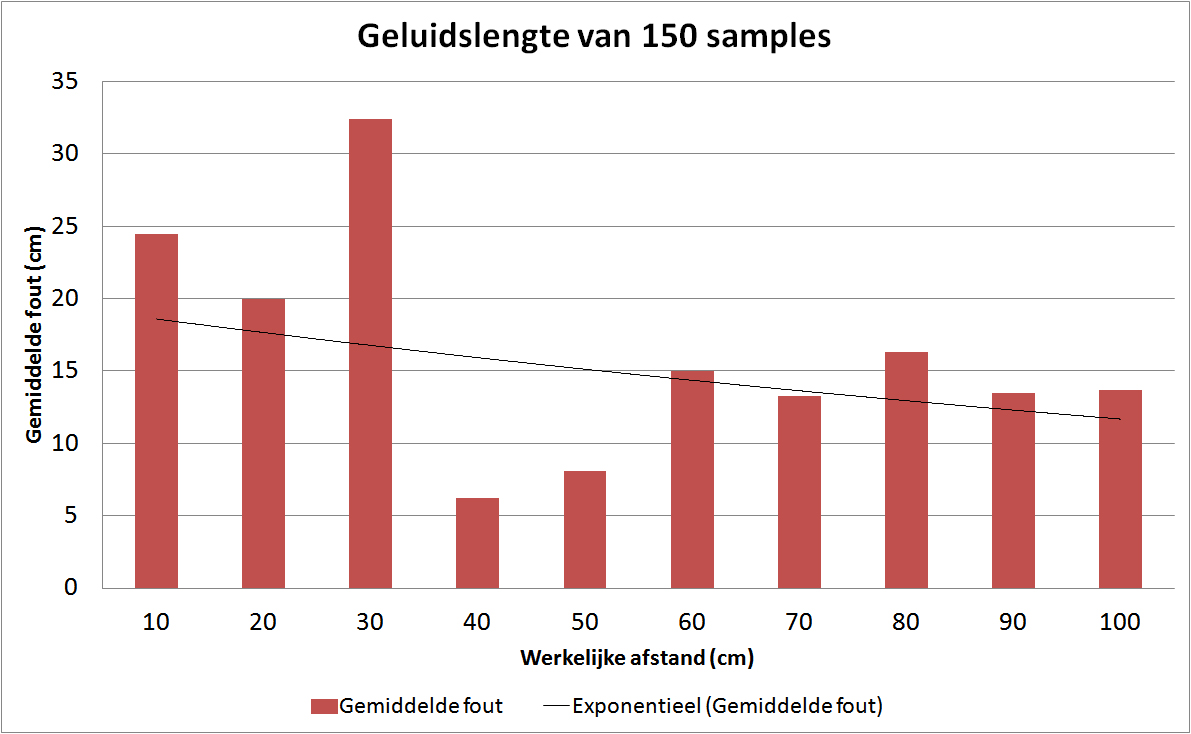
\includegraphics[scale=0.4]{150-samples}
\caption{gemiddelde fout bij piepgeluid met geluidslengte van 150 samples.}
\label{fig:150}
\end{figure}

\section{Resultaten}
\label{sec:resultaten}
Figuur \ref{fig:150} en \ref{fig:300} tonen de gemiddelde fouten bij de afstandsmetingen voor geluidslengtes van respectievelijk 150 en 300 samples.

Alle geregistreerde afstandsmetingen waren in drie verschillende klassen ingedeeld. In figuur \ref{fig:classi} wordt weergegeven dat 25\% van alle metingen niet konden worden voltooid. Deze pogingen werden geclassificeerd als mislukt. Geslaagde metingen werden geclassificeerd op basis van precisie: 33\% van de metingen zaten binnen een foutmarge van 20\% en 42\% erbuiten.

\begin{figure}[t]
\centering
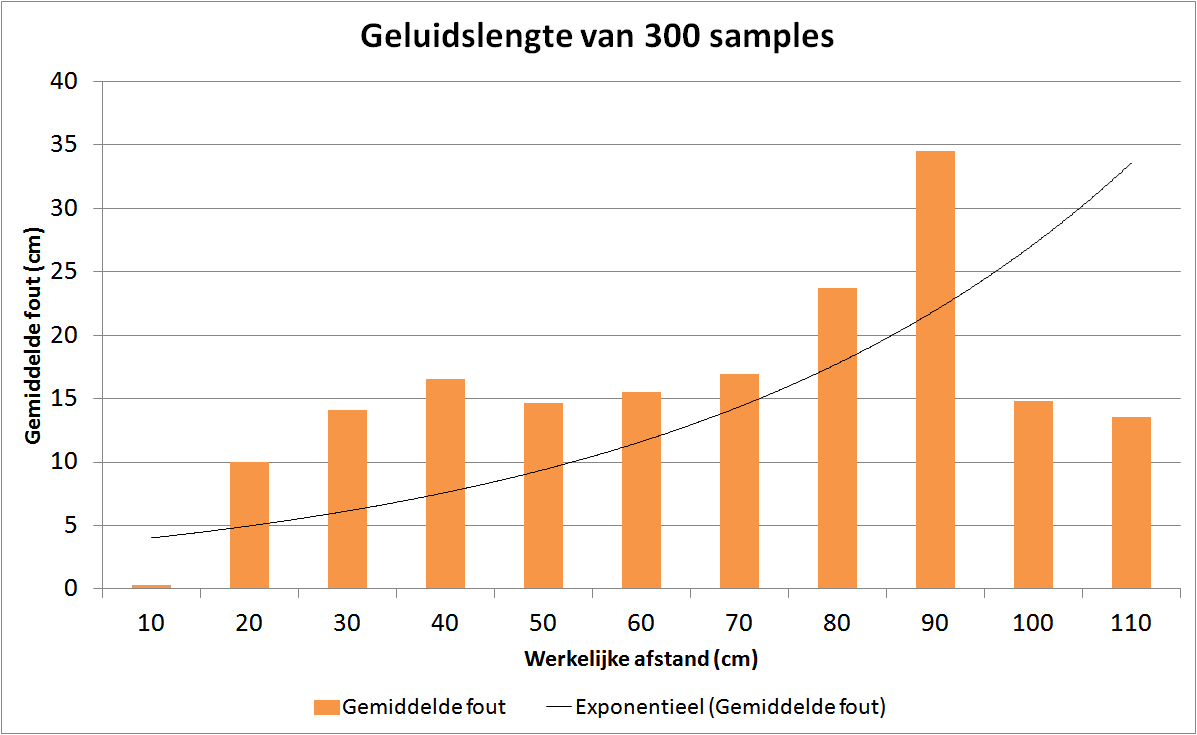
\includegraphics[scale=0.4]{300-samples}
\caption{gemiddelde fout bij piepgeluid met geluidslengte van 150 samples.}
\label{fig:300}
\end{figure}

Het aantal metingen dat correct is binnen een foutmarge van 10 cm is $21.7 \%$ en $23.3\%$ voor piepgeluiden met een lengte van respectievelijk 150 en 300 samples. 

\section{Discussie}
\label{sec:discussie}
Het meetproces is te fragiel gebleken en is niet geschikt voor nauwkeurige positie bepaling. Uit figuur blijkt dat 25\% van de afstandsmetingen mislukken, dit kan worden veroorzaakt doordat een piepgeluid ergens in het proces niet wordt herkend. Het missen van een piepgeluid kan wel worden herkend en het proces kan dan opnieuw worden opgestart. 

Uit de resultaten blijkt ook dat de geluidslengte invloed heeft op de prestaties van het systeem. Uit figuren \ref{fig:150} en \ref{fig:300} blijkt dat geluiden van een langere lengte op kortere afstanden beter presteren dan geluiden met een kortere lengte. De oorzaak hiervan kan nog niet worden gevonden. Er zijn meer experimenten hiervoor nodig, dit zou eventueel in een vervolgonderzoek kunnen worden uitgevoerd.

In voorgaand onderzoek \cite{qiu2011feasibility} waren in 90\% van de gevallen afstanden tot 13.9 cm nauwkeurig te meten. Onze hypothese was dat we een nauwkeurigheid van 10 cm zouden kunnen halen. Dit was alleen mogelijk in $16.7\%$ van de gevallen. De gebruikte materialen in dit onderzoek waren niet toereikend om tot dezelfde of betere resultaten gekomen. Een beter resultaat zou kunnen worden behaald door telefoons te gebruiken die over meerdere microfoons beschikken.

Realtime akoestische positiebepaling is zeker mogelijk met het juiste materiaal. De HTC Desire C toestellen lijken hier niet geschikt voor te zijn.

\section{Nawoord}
\label{sec:nawoord}
Mustafa had zich tijdens het project gericht op het audio gedeelte en Jos op het Bluetooth gedeelte.

\bibliographystyle{plain}
\bibliography{refs}

\end{document}


